
% TODO: Add proofs, implementation details, supplementary experiments, and
% complete prompts or protocols here.

\section{Related Work}

\subsection{Model Distillation}
Knowledge distillation is originally proposed as to transfer the capicity of a teacher model to a student model \cite{hinton2015distilling}. With rapid development of LLM, fine-tuning on teacher-generated data has become an increasingly important form of distillation, allowing student models to acquire advanced capabilities directly from the teacher's responses \cite{hsieh2023distilling, mukherjee2023orca}. This paradigm has also been extended to agent systems \cite{kang2026distilling, liu2026structured, luo2026agentark}. Agent Distillation \cite{kang2026distilling} proposed an agent distillation method that enables student model to learn both tool-use behaviors and reasoning capabilities. AgentArk \cite{luo2026agentark} introduced a method that distills multi-agent dynamics into the weights of a single model. Agent trajectories record not only generated text but also tool use and multi-step decisions, making them valuable supervision for distillation. As these trajectories can be used to cheaply transfer the capabilities of teacher agents, unauthorized distillation poses a growing threat to model copyright and calls for effective detection and tracing mechanisms.


\subsection{Model Watermarking}



\partitle{Content watermarking}
Recent studies have proposed a series of content watermarking methods to identify whether a given output is generated by a specific model. Early methods mainly embed statistical signals during token generation, such as the red-green list mechanism \cite{kirchenbauer2023watermark}. Later studies further improve the robustness and generation quality of watermarks by using semantic information \cite{liu2024semantic, huo2026pmark, huo2026samark,hou2024semstamp}. However, with the development of LLM agents, traditional content watermarks are difficult to directly apply to agent settings. These methods usually embed watermark signals by changing token choices or semantic expressions in free-form text, while the key outputs of agents are often tool calls with strict format requirements. Directly modifying these outputs may break the tool calls and affect correct execution. Therefore, recent studies have started to move watermarks from generated content to agent trajectories and behavior patterns \cite{huang2025agent, an2026sequential, zhang2026memmark}.


\partitle{Model watermarking against distillation}
Several watermarking methods have been proposed to protect models against unauthorized distillation. Methods such as Lexical Watermark and CATER insert special word patterns into teacher outputs, so that student models trained on these outputs can inherit detectable features~\cite{he2022protecting, he2022cater, yang2026asking}. Recent work further targets LLM distillation by changing token generation or rewriting reasoning traces, either reducing the value of teacher outputs for distillation or leaving detectable signals in the student model~\cite{savani2026antidistillation, xu2026antidistillation, ma2026protecting}. However, these methods mainly work on text tokens or reasoning traces, and are difficult to directly apply to agents whose behavior is mainly represented by structured tool calls and multi-step interactions. Recent work has extended anti-distillation watermarking to agent trajectories~\cite{wang2026protecting}, but its main evaluation still focuses on settings where the teacher and student models use the same base model, and its robustness to data processing such as data mixing remains limited. Therefore, a more general and robust watermarking method is still needed for tracing agent distillation.




\section{Supplement of Experiments}


\subsection{Experimental Details}
\label{sec:experimental-details}

\partitle{Hyperparameter selection} We select \name{} hyperparameters through preliminary experiments to balance stealthiness, utility and detection reliability. For dynamic scheduling, we set $p_0 = 0.1$, $\Delta p = 0.1$, $p_{\mathtt{max}} = 0.5$, and the maximum budget $B = 10$. The system generates $K = 3$ candidates, and the scoring weights in Eq.~\ref{equ:score} are $\alpha = 0.35$, $\beta = 0.25$, and $\gamma = 0.40$. The repeatability score is $s_{\mathtt{rep}}^j=0$ for $n_j=0$, $0.6$ for $1\leq n_j<5$, and $1$ for $n_j\geq5$. For detection, we generate $N = 3$ parameterized variants per card and use a significance level $p=0.05$ with margin threshold $r=0.05$. For trace-level attribution in Eq.~\ref{eq:trace-score}, we set $\alpha' = 0.25$, $\beta' = 0.10$, and $\gamma' = 0.10$.



\partitle{Baselines} We evaluate our approach against two representative agent watermarking baselines. We exclude large language model antidistillation watermarks~\cite{xu2026antidistillation,savani2026antidistillation} from our comparison, as agent environments demand formatted outputs and modifying tokens or reasoning traces can cause format corruption and execution failures. Thus, we focus on agent schemes~\cite{an2026sequential,huang2025agent,luo2026agentark}. We select Seqwm~\cite{an2026sequential} and Agentwm~\cite{wang2026protecting} because Seqwm demonstrates better robustness among trace watermarks generated for agents, and Agentwm specifically targets agent anti-distillation. Their available implementations use different watermark encodings, test units, and decision statistics from \name{}; we therefore report each baseline in its native metric. Specifically, we train the student models $\mathcal{M}_s$ using the distillation dataset $\mathcal{D}_c$ watermarked by each respective scheme, and then have them replay 100 tasks from the set $\mathcal{S}$. For Agentwm, we collect unwatermarked traces using four distinct models to estimate the natural initial distribution $P_c$ of synonymous tool sets. The scheme then modifies this $P_c$ into a watermarked distribution $P_{\mathtt{wm}}$. During detection, it extracts 5 fixed synonymous tool sets (referred to as passes) from the 100 task replays. A pass is considered successfully detected only when the JSD between the student's empirical distribution and the distribution $P_{\mathtt{wm}}$ is at most 0.015. The student model is flagged as significant only if at least 3 out of 5 passes are detected ($\geq 3/5$). For Seqwm, it evaluates each replayed trace against a background null distribution generated from 1,000 incorrect keys. It uses the median $p$-value of these 100 test traces to determine whether the student model $\mathcal{M}_s$ is distilled, requiring a median $p < 0.05$ for a successful detection.



\subsection{Supplementary Effectiveness Results}
\label{sec:supplementary-effectiveness}
\begin{table*}[!t]
\centering
\setlength{\tabcolsep}{3.5pt}
\caption{Supplementary true-positive results for SWE-bench and Telecom.
Cards is the number of cards; hit-rate cells report hits / probes (rate).
$w/\ell$ gives card-level real / fake wins.
The Sig. column indicates statistical significance:
{\color{green}$\checkmark$} denotes $p < 0.05$,
whereas {\color{red}$\times$} denotes $p \ge 0.05$.}
\label{tab:appendix-true-positive}

\scriptsize
\begin{tabular}{l l c l | c c c c c}
\noalign{\hrule height 1.5pt}
\multirow{2}{*}{\textbf{Teacher Agent$\mathcal{M}_t$}} & \multirow{2}{*}{\textbf{Dataset}} & \multirow{2}{*}{\textbf{Cards}} & \multirow{2}{*}{\textbf{Student Model $\mathcal{M}_s$}} & \multicolumn{5}{c}{\textbf{Detection Results}} \\
\cline{5-9}
& & & & \textbf{$R^{\mathtt{real}}$ (\%)} & \textbf{$R^{\mathtt{fake}}$ (\%)} & \textbf{$w/\ell$} & \textbf{$p$-value} & \textbf{Sig.} \\
\hline
\multirow{8}{*}{GPT-OSS-120B} & \multirow{4}{*}{SWE-bench} & \multirow{4}{*}{274} & Mistral-24B & \tableRate{60}{387}{15.5} & \tableRate{18}{387}{4.7} & 46 / 6 & \tablePval{5.2}{-9} & {\color{green}\checkmark} \\
& & & GLM-4.7-Flash & \tableRate{81}{387}{20.9} & \tableRate{21}{387}{5.4} & 67 / 6 & \tablePval{2.0}{-14} & {\color{green}\checkmark} \\
& & & Qwen3-14B & \tableRate{67}{387}{17.3} & \tableRate{18}{387}{4.7} & 54 / 4 & \tablePval{1.6}{-12} & {\color{green}\checkmark} \\
& & & Qwen3-32B & \tableRate{72}{387}{18.6} & \tableRate{20}{387}{5.2} & 58 / 6 & \tablePval{4.5}{-12} & {\color{green}\checkmark} \\
\cline{2-9}
& \multirow{4}{*}{Telecom} & \multirow{4}{*}{125} & Mistral-24B & \tableRate{83}{146}{56.8} & \tableRate{46}{146}{31.5} & 44 / 7 & \tablePval{6.1}{-8} & {\color{green}\checkmark} \\
& & & GLM-4.7-Flash & \tableRate{76}{146}{52.1} & \tableRate{42}{146}{28.8} & 42 / 4 & \tablePval{2.6}{-9} & {\color{green}\checkmark} \\
& & & Qwen3-14B & \tableRate{86}{146}{58.9} & \tableRate{44}{146}{30.1} & 48 / 6 & \tablePval{1.6}{-9} & {\color{green}\checkmark} \\
& & & Qwen3-32B & \tableRate{85}{146}{58.2} & \tableRate{36}{146}{24.7} & 57 / 7 & \tablePval{3.8}{-11} & {\color{green}\checkmark} \\
\hline
\multirow{8}{*}{Kimi-K2.5} & \multirow{4}{*}{SWE-bench} & \multirow{4}{*}{262} & Mistral-24B & \tableRate{85}{437}{19.5} & \tableRate{50}{437}{11.4} & 38 / 9 & \tablePval{1.2}{-5} & {\color{green}\checkmark} \\
& & & GLM-4.7-Flash & \tableRate{80}{437}{18.3} & \tableRate{42}{437}{9.6} & 34 / 5 & \tablePval{1.2}{-6} & {\color{green}\checkmark} \\
& & & Qwen3-14B & \tableRate{48}{437}{11.0} & \tableRate{17}{437}{3.9} & 33 / 8 & \tablePval{5.6}{-5} & {\color{green}\checkmark} \\
& & & Qwen3-32B & \tableRate{45}{437}{10.3} & \tableRate{14}{437}{3.2} & 27 / 1 & \tablePval{1.1}{-7} & {\color{green}\checkmark} \\
\cline{2-9}
& \multirow{4}{*}{Telecom} & \multirow{4}{*}{122} & Mistral-24B & \tableRate{68}{192}{35.4} & \tableRate{48}{192}{25.0} & 37 / 14 & \tablePval{8.8}{-4} & {\color{green}\checkmark} \\
& & & GLM-4.7-Flash & \tableRate{56}{192}{29.2} & \tableRate{28}{192}{14.6} & 33 / 6 & \tablePval{7.1}{-6} & {\color{green}\checkmark} \\
& & & Qwen3-14B & \tableRate{60}{192}{31.2} & \tableRate{36}{192}{18.8} & 33 / 9 & \tablePval{1.4}{-4} & {\color{green}\checkmark} \\
& & & Qwen3-32B & \tableRate{66}{192}{34.4} & \tableRate{43}{192}{22.4} & 27 / 6 & \tablePval{1.6}{-4} & {\color{green}\checkmark} \\
\noalign{\hrule height 1.5pt}
\end{tabular}
\end{table*}


\begin{table*}[!t]
\centering
\setlength{\tabcolsep}{3.5pt}
\caption{Supplementary false-positive results for SWE-bench and Telecom.
Cards is the number of cards; hit-rate cells report hits / probes (rate).
$w/\ell$ gives card-level real / fake wins.
The Sig. column indicates statistical significance:
{\color{green}$\checkmark$} denotes $p < 0.05$,
whereas {\color{red}$\times$} denotes $p \ge 0.05$.}
\label{tab:appendix-false-positive}

\scriptsize
\begin{tabular}{l l c l | c c c c c}
\noalign{\hrule height 1.5pt}
\multirow{2}{*}{\textbf{Teacher Agent$\mathcal{M}_t$}} & \multirow{2}{*}{\textbf{Dataset}} & \multirow{2}{*}{\textbf{Cards}} & \multirow{2}{*}{\textbf{Clean Model $\mathcal{M}_c$}} & \multicolumn{5}{c}{\textbf{Detection Results}} \\
\cline{5-9}
& & & & \textbf{$R^{\mathtt{real}}$ (\%)} & \textbf{$R^{\mathtt{fake}}$ (\%)} & \textbf{$w/\ell$} & \textbf{$p$-value} & \textbf{Sig.} \\
\hline
\multirow{16}{*}{GPT-OSS-120B} & \multirow{8}{*}{SWE-bench} & \multirow{8}{*}{274} & DeepSeek-V4-Flash & \tableRate{0}{387}{0.0} & \tableRate{0}{387}{0.0} & 0 / 0 & \tablePval{1.0}{0} & {\color{red}$\times$} \\
& & & MiniMax-M2.5 & \tableRate{5}{387}{1.3} & \tableRate{2}{387}{0.5} & 4 / 1 & \tablePval{1.9}{-1} & {\color{red}$\times$} \\
& & & Mistral-24B & \tableRate{15}{387}{3.9} & \tableRate{10}{387}{2.6} & 10 / 6 & \tablePval{2.3}{-1} & {\color{red}$\times$} \\
& & & Qwen3-14B & \tableRate{0}{387}{0.0} & \tableRate{3}{387}{0.8} & 0 / 3 & \tablePval{1.0}{0} & {\color{red}$\times$} \\
& & & Qwen3-32B & \tableRate{0}{387}{0.0} & \tableRate{2}{387}{0.5} & 0 / 2 & \tablePval{1.0}{0} & {\color{red}$\times$} \\
& & & Qwen3.5-Flash & \tableRate{4}{387}{1.0} & \tableRate{5}{387}{1.3} & 4 / 3 & \tablePval{5.0}{-1} & {\color{red}$\times$} \\
& & & MiMo-V2.5 & \tableRate{3}{387}{0.8} & \tableRate{3}{387}{0.8} & 2 / 2 & \tablePval{6.9}{-1} & {\color{red}$\times$} \\
& & & GLM-4.7-Flash & \tableRate{1}{387}{0.3} & \tableRate{2}{387}{0.5} & 1 / 2 & \tablePval{8.8}{-1} & {\color{red}$\times$} \\
\cline{2-9}
& \multirow{8}{*}{Telecom} & \multirow{8}{*}{125} & DeepSeek-V4-Flash & \tableRate{18}{146}{12.3} & \tableRate{13}{146}{8.9} & 10 / 5 & \tablePval{1.5}{-1} & {\color{red}$\times$} \\
& & & MiniMax-M2.5 & \tableRate{21}{146}{14.4} & \tableRate{19}{146}{13.0} & 6 / 3 & \tablePval{2.5}{-1} & {\color{red}$\times$} \\
& & & Mistral-24B & \tableRate{11}{146}{7.5} & \tableRate{9}{146}{6.2} & 6 / 5 & \tablePval{5.0}{-1} & {\color{red}$\times$} \\
& & & Qwen3-14B & \tableRate{17}{146}{11.6} & \tableRate{21}{146}{14.4} & 3 / 6 & \tablePval{9.1}{-1} & {\color{red}$\times$} \\
& & & Qwen3-32B & \tableRate{17}{146}{11.6} & \tableRate{18}{146}{12.3} & 2 / 3 & \tablePval{8.1}{-1} & {\color{red}$\times$} \\
& & & Qwen3.5-Flash & \tableRate{11}{146}{7.5} & \tableRate{8}{146}{5.5} & 6 / 3 & \tablePval{2.5}{-1} & {\color{red}$\times$} \\
& & & MiMo-V2.5 & \tableRate{13}{146}{8.9} & \tableRate{13}{146}{8.9} & 8 / 8 & \tablePval{6.0}{-1} & {\color{red}$\times$} \\
& & & GLM-4.7-Flash & \tableRate{1}{146}{0.7} & \tableRate{0}{146}{0.0} & 1 / 0 & \tablePval{5.0}{-1} & {\color{red}$\times$} \\
\hline
\multirow{16}{*}{Kimi-K2.5} & \multirow{8}{*}{SWE-bench} & \multirow{8}{*}{262} & DeepSeek-V4-Flash & \tableRate{12}{437}{2.7} & \tableRate{5}{437}{1.1} & 8 / 3 & \tablePval{1.1}{-1} & {\color{red}$\times$} \\
& & & MiniMax-M2.5 & \tableRate{14}{437}{3.2} & \tableRate{7}{437}{1.6} & 9 / 4 & \tablePval{1.3}{-1} & {\color{red}$\times$} \\
& & & Mistral-24B & \tableRate{20}{437}{4.6} & \tableRate{11}{437}{2.5} & 10 / 4 & \tablePval{9.0}{-2} & {\color{red}$\times$} \\
& & & Qwen3-14B & \tableRate{1}{437}{0.2} & \tableRate{1}{437}{0.2} & 1 / 1 & \tablePval{7.5}{-1} & {\color{red}$\times$} \\
& & & Qwen3-32B & \tableRate{2}{437}{0.5} & \tableRate{2}{437}{0.5} & 2 / 2 & \tablePval{6.9}{-1} & {\color{red}$\times$} \\
& & & Qwen3.5-Flash & \tableRate{15}{437}{3.4} & \tableRate{13}{437}{3.0} & 6 / 4 & \tablePval{3.8}{-1} & {\color{red}$\times$} \\
& & & MiMo-V2.5 & \tableRate{10}{437}{2.3} & \tableRate{6}{437}{1.4} & 8 / 5 & \tablePval{2.9}{-1} & {\color{red}$\times$} \\
& & & GLM-4.7-Flash & \tableRate{5}{437}{1.1} & \tableRate{1}{437}{0.2} & 4 / 0 & \tablePval{6.2}{-2} & {\color{red}$\times$} \\
\cline{2-9}
& \multirow{8}{*}{Telecom} & \multirow{8}{*}{122} & DeepSeek-V4-Flash & \tableRate{11}{192}{5.7} & \tableRate{8}{192}{4.2} & 4 / 1 & \tablePval{1.9}{-1} & {\color{red}$\times$} \\
& & & MiniMax-M2.5 & \tableRate{23}{192}{12.0} & \tableRate{18}{192}{9.4} & 9 / 5 & \tablePval{2.1}{-1} & {\color{red}$\times$} \\
& & & Mistral-24B & \tableRate{19}{192}{9.9} & \tableRate{16}{192}{8.3} & 14 / 11 & \tablePval{3.5}{-1} & {\color{red}$\times$} \\
& & & Qwen3-14B & \tableRate{10}{192}{5.2} & \tableRate{8}{192}{4.2} & 7 / 5 & \tablePval{3.9}{-1} & {\color{red}$\times$} \\
& & & Qwen3-32B & \tableRate{10}{192}{5.2} & \tableRate{5}{192}{2.6} & 6 / 1 & \tablePval{6.2}{-2} & {\color{red}$\times$} \\
& & & Qwen3.5-Flash & \tableRate{9}{192}{4.7} & \tableRate{3}{192}{1.6} & 6 / 1 & \tablePval{6.2}{-2} & {\color{red}$\times$} \\
& & & MiMo-V2.5 & \tableRate{10}{192}{5.2} & \tableRate{7}{192}{3.6} & 6 / 4 & \tablePval{3.8}{-1} & {\color{red}$\times$} \\
& & & GLM-4.7-Flash & \tableRate{1}{192}{0.5} & \tableRate{0}{192}{0.0} & 1 / 0 & \tablePval{5.0}{-1} & {\color{red}$\times$} \\
\noalign{\hrule height 1.5pt}
\end{tabular}
\end{table*}

\partitle{Trace-level detection} After a successful model-level detection, we further examine whether \name{} can identify the specific trajectories in the suspicious set $\mathcal{S}$ that are most likely used for distillation. We separately rank the scores $S_\tau$ of the 100 trajectories from $\mathcal{S}$ on the four student models and report the arithmetic mean of $\operatorname{\mathtt{Precision}}@K$ across the four students in Table~\ref{tab:trace-attribution}. The overall average precision across the six cohorts remains at least $82.1\%$ for every reported $K$. SWE-bench--GPT achieves a perfect $100.0\%$ at P@10. These results show that \name{} can identify the specific leaked data with high precision across all six cohorts.

\begin{table*}[!t]
\centering
\caption{Trace-level attribution accuracy. Each entry is the arithmetic mean of $\operatorname{\mathtt{Precision}}@K$ over the four student models in the cohort.}
\label{tab:trace-attribution}
\small
\setlength{\tabcolsep}{5.5pt}
\begin{tabular*}{\linewidth}{@{\extracolsep{\fill}}l l | c c c c c@{}}
\noalign{\hrule height 1.5pt}
\textbf{Teacher Agent $\mathcal{M}_t$} & \textbf{Dataset} & \textbf{P@10} & \textbf{P@15} & \textbf{P@20} & \textbf{P@25} & \textbf{P@30} \\
\hline
\multirow{3}{*}{GPT-OSS-120B} & BFCL & 72.5\% & 80.0\% & 80.0\% & 79.0\% & 81.7\% \\
& SWE-bench & 100.0\% & 98.3\% & 96.2\% & 96.0\% & 94.2\% \\
& Telecom & 75.0\% & 78.3\% & 80.0\% & 82.0\% & 84.2\% \\
\hline
\multirow{3}{*}{Kimi-K2.5} & BFCL & 82.5\% & 81.7\% & 82.5\% & 84.0\% & 80.8\% \\
& SWE-bench & 85.0\% & 86.7\% & 86.2\% & 82.0\% & 80.8\% \\
& Telecom & 80.0\% & 83.3\% & 82.5\% & 75.0\% & 70.8\% \\
\hline
\multicolumn{2}{l|}{\textbf{Overall average}} & \textbf{82.5\%} & \textbf{84.7\%} & \textbf{84.6\%} & \textbf{83.0\%} & \textbf{82.1\%} \\
\noalign{\hrule height 1.5pt}
\end{tabular*}
\end{table*}

\partitle{Impact on identification accuracy} To evaluate the impact of identification accuracy on detection accuracy, we simulate different training shares by resampling our empirical results. In practice, upstream traffic monitoring is often tuned for high recall to avoid missing distillation requests, which can introduce additional benign or unrelated trajectories into the suspicious set $\mathcal{S}$. We test \name{} under lower shares down to 10\%. Specifically, we divide the evaluated cards for each cohort and student model into trained and untrained groups. Next, we estimate their outcome distributions and resample these two groups at various target ratios. The $50\%$ share serves as the observed baseline. For other simulated shares, we perform 2,000 independent draws and apply the same one-sided exact sign test. As shown in Figure~\ref{fig:training-share-sensitivity}, which reports the median $p$-value, all 24 settings remain significant at a $20\%$ training share. At $10\%$, 21 of 24 settings remain significant.


\begin{figure*}[!t]
\centering
\begin{subfigure}[t]{0.32\textwidth}
\centering
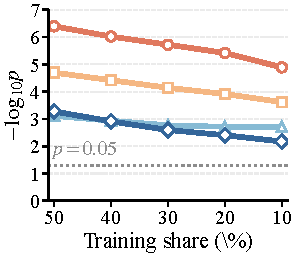
\includegraphics[width=0.82\linewidth]{figure/training_share_bfcl_gpt.pdf}
\caption{BFCL / GPT}
\end{subfigure}\hfill
\begin{subfigure}[t]{0.32\textwidth}
\centering
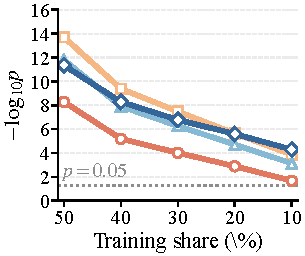
\includegraphics[width=0.82\linewidth]{figure/training_share_swe_bench_gpt.pdf}
\caption{SWE-bench / GPT-OSS-120B}
\end{subfigure}\hfill
\begin{subfigure}[t]{0.32\textwidth}
\centering
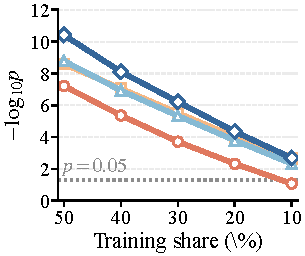
\includegraphics[width=0.82\linewidth]{figure/training_share_telecom_gpt.pdf}
\caption{Telecom / GPT}
\end{subfigure}

\begin{subfigure}[t]{0.32\textwidth}
\centering
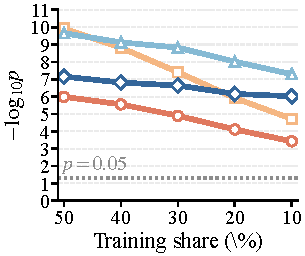
\includegraphics[width=0.82\linewidth]{figure/training_share_bfcl_kimi.pdf}
\caption{BFCL / Kimi}
\end{subfigure}\hfill
\begin{subfigure}[t]{0.32\textwidth}
\centering
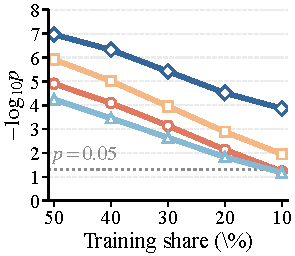
\includegraphics[width=0.82\linewidth]{figure/training_share_swe_bench_kimi.pdf}
\caption{SWE-bench / Kimi-K2.5}
\end{subfigure}\hfill
\begin{subfigure}[t]{0.32\textwidth}
\centering
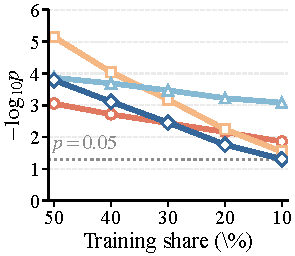
\includegraphics[width=0.82\linewidth]{figure/training_share_telecom_kimi.pdf}
\caption{Telecom / Kimi}
\end{subfigure}
\caption{
Impact of identification accuracy. The horizontal axis denotes the training share and the vertical axis denotes $-\log_{10}p$, where larger values indicate stronger evidence. In (a)--(f), the colored lines and hollow markers denote student models: \textcolor[HTML]{E0795F}{\rule[0.5ex]{0.5em}{1.5pt}\hspace{0.08em}$\circ$\hspace{0.08em}\rule[0.5ex]{0.5em}{1.5pt}} Mistral-24B, \textcolor[HTML]{F5B783}{\rule[0.5ex]{0.5em}{1.5pt}\hspace{0.08em}$\square$\hspace{0.08em}\rule[0.5ex]{0.5em}{1.5pt}} GLM-4.7-Flash, \textcolor[HTML]{86BAD4}{\rule[0.5ex]{0.5em}{1.5pt}\hspace{0.08em}$\triangle$\hspace{0.08em}\rule[0.5ex]{0.5em}{1.5pt}} Qwen3-14B, and \textcolor[HTML]{34669A}{\rule[0.5ex]{0.5em}{1.5pt}\hspace{0.08em}$\diamond$\hspace{0.08em}\rule[0.5ex]{0.5em}{1.5pt}} Qwen3-32B. The \textcolor[HTML]{8C8C8C}{\hdashrule[0.5ex]{1.2em}{1.2pt}{1pt 1.5pt}}  marks $p=0.05$.
}
\label{fig:training-share-sensitivity}
\end{figure*}


\subsection{Supplementary of Robustness}
\label{sec:supplementary-robustness}
\begin{figure*}[!t]
\centering
\begin{subfigure}[t]{\robustnessPanelWidth}
\centering
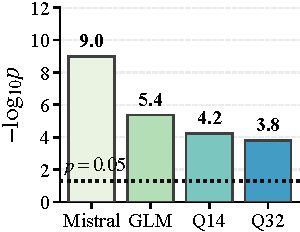
\includegraphics[width=0.72\linewidth]{figure/robustness_data_flooding_plus_bfcl_r1.pdf}
\caption{BFCL: R1}
\end{subfigure}\hfill
\begin{subfigure}[t]{\robustnessPanelWidth}
\centering
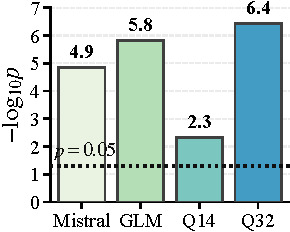
\includegraphics[width=0.72\linewidth]{figure/robustness_data_flooding_plus_bfcl_r2.pdf}
\caption{BFCL: R2}
\end{subfigure}\hfill
\begin{subfigure}[t]{\robustnessPanelWidth}
\centering
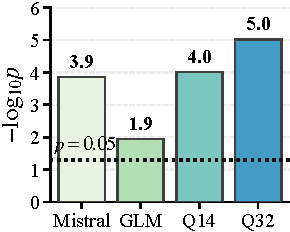
\includegraphics[width=0.72\linewidth]{figure/robustness_data_flooding_plus_bfcl_r3.pdf}
\caption{BFCL: R3}
\end{subfigure}\par
\begin{subfigure}[t]{\robustnessPanelWidth}
\centering
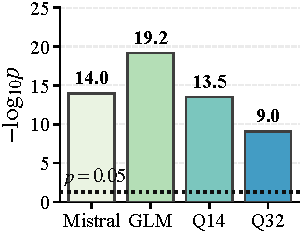
\includegraphics[width=0.72\linewidth]{figure/robustness_data_flooding_plus_swe_bench_r1.pdf}
\caption{SWE-bench: R1}
\end{subfigure}\hfill
\begin{subfigure}[t]{\robustnessPanelWidth}
\centering
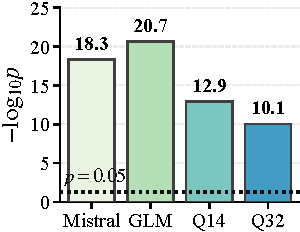
\includegraphics[width=0.72\linewidth]{figure/robustness_data_flooding_plus_swe_bench_r2.pdf}
\caption{SWE-bench: R2}
\end{subfigure}\hfill
\begin{subfigure}[t]{\robustnessPanelWidth}
\centering
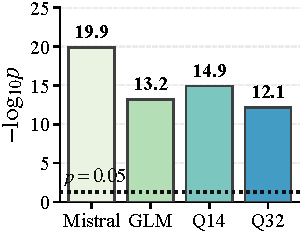
\includegraphics[width=0.72\linewidth]{figure/robustness_data_flooding_plus_swe_bench_r3.pdf}
\caption{SWE-bench: R3}
\end{subfigure}
\caption{Advanced data flooding robustness. The horizontal axis lists the four student models and the vertical axis reports $-\log_{10}p$. In (a)--(f), \robustnessModelLegend. The \textcolor[HTML]{8C8C8C}{\hdashrule[0.5ex]{1.2em}{1.2pt}{1pt 1.5pt}} marks $p=0.05$.}
\label{fig:data-flooding-plus-robustness}
\end{figure*}

\partitle{Advanced data flooding} An attacker may build a diverse training set by collecting solutions to the same tasks from different teacher agents to improve the distilled model's performance~\cite{cui2023ultrafeedback, luo2026agentark}, which also dilutes the watermark signals. To evaluate the robustness of \name{} against this advanced data flooding tactic, we mix the original watermarked dataset $\mathcal{D}_c$ with clean trajectories generated by alternative teacher agents. Specifically, we sequentially introduce clean data from DeepSeek-V4-Flash, MiMo-V2.5, and Qwen3-235B-A22B. In the R1, R2, and R3 settings, we incorporate data from 1, 2, and 3 alternative teachers, resulting in ratios of $1{:}1$, $1{:}2$, and $1{:}3$. Then we use the combined dataset to train the student models and detect their watermarks. We evaluate a total of 24 settings across BFCL and SWE-bench, 3 dilution ratios, and 4 student models. As shown in Figure~\ref{fig:data-flooding-plus-robustness}, \name{} successfully detects every setting. Even under the most challenging R3 setting, all 8 tested student models remain successfully detected.



\partitle{Truncation} Before distillation, an attacker may truncate the trailing tokens of the interaction trajectories to fit the student models' context length limits or to deliberately disrupt potential watermark signals~\cite{kirchenbauer2023watermark}. To evaluate the robustness against this operation, we remove 10\%, 15\%, and 20\% of the tokens from the tail of each watermarked training sequence, and train the student models using these truncated trajectories. We evaluate a total of 24 settings across the BFCL and SWE-bench benchmarks, 3 truncation levels (T10, T15, and T20), and 4 student models. As shown in Figure~\ref{fig:truncation-robustness}, \name{} successfully detects the watermark in every setting. Even under the most aggressive T20 truncation setting, all 8 tested student models remain successfully detected.
\begin{figure*}[!t]
\centering
\begin{subfigure}[t]{\robustnessPanelWidth}
\centering
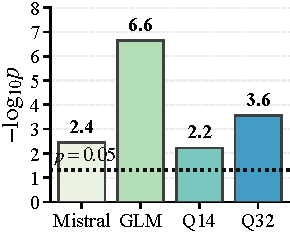
\includegraphics[width=0.72\linewidth]{figure/robustness_truncation_bfcl_t10.pdf}
\caption{BFCL: T10}
\end{subfigure}\hfill
\begin{subfigure}[t]{\robustnessPanelWidth}
\centering
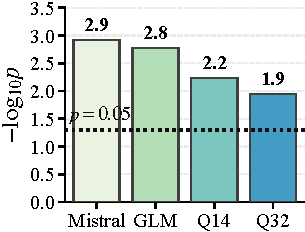
\includegraphics[width=0.72\linewidth]{figure/robustness_truncation_bfcl_t15.pdf}
\caption{BFCL: T15}
\end{subfigure}\hfill
\begin{subfigure}[t]{\robustnessPanelWidth}
\centering
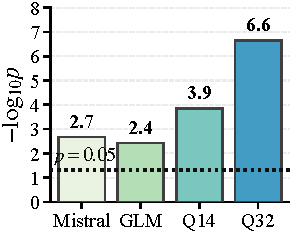
\includegraphics[width=0.72\linewidth]{figure/robustness_truncation_bfcl_t20.pdf}
\caption{BFCL: T20}
\end{subfigure}\par
\begin{subfigure}[t]{\robustnessPanelWidth}
\centering
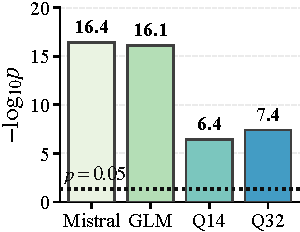
\includegraphics[width=0.72\linewidth]{figure/robustness_truncation_swe_bench_t10.pdf}
\caption{SWE-bench: T10}
\end{subfigure}\hfill
\begin{subfigure}[t]{\robustnessPanelWidth}
\centering
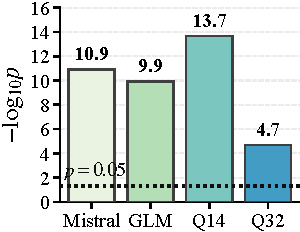
\includegraphics[width=0.72\linewidth]{figure/robustness_truncation_swe_bench_t15.pdf}
\caption{SWE-bench: T15}
\end{subfigure}\hfill
\begin{subfigure}[t]{\robustnessPanelWidth}
\centering
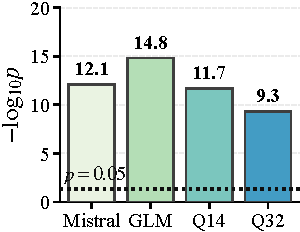
\includegraphics[width=0.72\linewidth]{figure/robustness_truncation_swe_bench_t20.pdf}
\caption{SWE-bench: T20}
\end{subfigure}
\caption{Truncation robustness. The horizontal axis lists the four student models and the vertical axis reports $-\log_{10}p$ . In (a)--(f), \robustnessModelLegend. The \textcolor[HTML]{8C8C8C}{\hdashrule[0.5ex]{1.2em}{1.2pt}{1pt 1.5pt}} marks $p=0.05$.}
\label{fig:truncation-robustness}
\end{figure*}

\begin{table}[!t]
\centering
\caption{Agentwm robustness to data flooding.}
\label{tab:baseline-robustness}
\scriptsize
\setlength{\tabcolsep}{4pt}
\begin{tabular*}{\linewidth}{@{\extracolsep{\fill}}l l | c c@{}}
\noalign{\hrule height 1.5pt}
\textbf{Dataset} & \textbf{Student Model $\mathcal{M}_s$} & \textbf{D1} & \textbf{D5} \\
\hline
\multirow{4}{*}{BFCL} & Mistral-24B & $0/5$ {\color{red}$\times$} & $0/5$ {\color{red}$\times$} \\
& GLM-4.7-Flash & $0/5$ {\color{red}$\times$} & $0/5$ {\color{red}$\times$} \\
& Qwen3-14B & $2/5$ {\color{red}$\times$} & $0/5$ {\color{red}$\times$} \\
& Qwen3-32B & $1/5$ {\color{red}$\times$} & $0/5$ {\color{red}$\times$} \\
\hline
\multirow{4}{*}{SWE-bench} & Mistral-24B & $1/5$ {\color{red}$\times$} & $1/5$ {\color{red}$\times$} \\
& GLM-4.7-Flash & $2/5$ {\color{red}$\times$} & $0/5$ {\color{red}$\times$} \\
& Qwen3-14B & $0/5$ {\color{red}$\times$} & $1/5$ {\color{red}$\times$} \\
& Qwen3-32B & $0/5$ {\color{red}$\times$} & $1/5$ {\color{red}$\times$} \\
\noalign{\hrule height 1.5pt}
\end{tabular*}
\end{table}
\partitle{Baseline robustness} Since Seqwm does not successfully detect distilled students(Table~\ref{tab:baseline-effectiveness}), we focus our robustness evaluation on Agentwm under data flooding (the D1 and D5 settings). To ensure a rigorous comparison, we process the clean standard data to match the initial distribution $P_c$ before mixing it with the watermarked traces. As shown in Table~\ref{tab:baseline-robustness}, all 16 evaluated settings fail to meet Agentwm's $\geq 3/5$ detection threshold. Agentwm encodes its watermark by shifting the tool-variant distribution towards $P_{\mathtt{wm}}$. By flooding the training corpus with clean trajectories calibrated to $P_c$, the overall frequencies are pulled back towards the unwatermarked state. This directly dilutes the artificial distributional signal, resulting in the distilled students not sufficiently reproducing the watermarked patterns for reliable detection.



\section{Discussion on Statistical Test}

\begin{table*}[!t]
\centering
\caption{Comparison of representative anti-distillation methods.}
\label{tab:anti-distillation-comparison}
\begin{threeparttable}
\scriptsize
% Spacing controls: increase/decrease these two values as needed.
\setlength{\tabcolsep}{2.5pt}       % horizontal (column) spacing
\renewcommand{\arraystretch}{1.08}  % vertical (row) spacing

\begin{tabular}{@{}
    >{\raggedright\arraybackslash}p{1.60cm}
    >{\raggedright\arraybackslash}p{2.1cm}
    >{\raggedright\arraybackslash}p{1.70cm}
    >{\centering\arraybackslash}p{0.90cm}
    >{\raggedright\arraybackslash}p{1.8cm}
    >{\centering\arraybackslash}p{0.75cm}
    >{\centering\arraybackslash}p{0.70cm}
    >{\centering\arraybackslash}p{0.75cm}
    >{\raggedright\arraybackslash}p{6.45cm}@{}}
\noalign{\hrule height 1.5pt}
\multirow{2}{1.60cm}{\textbf{Family}} &
\multirow{2}{2.1cm}{\textbf{Shared limits}} &
\multirow{2}{1.70cm}{\textbf{Method}} &
\multirow{2}{0.90cm}{\centering\textbf{Acc.}} &
\multirow{2}{1.8cm}{\textbf{Audit prior}} &
\multicolumn{2}{c}{\textbf{Cost}} &
\multirow{2}{0.75cm}{\centering\textbf{Evid.}} &
\multirow{2}{6.45cm}{\textbf{Main limitation}} \\
\cline{6-7}
& & & & & \textbf{Inject.} & \textbf{Verify} & & \\
\hline

\multirow[c]{5}{1.60cm}{\raggedright Watermarking} &
\multirow[c]{5}{2.15cm}{\raggedright
Limited robustness; additional cost.} &
ADFP &
BB &
Same tasks &
High &
Med. &
Strong &
High cost; sensitive to data dilution; utility loss$^{\star}$.\\

& &
AgentWM &
BB &
Same domain &
Low &
High &
Strong &
Weak cross-model robustness$^{\star}$; sensitive to data dilution$^{\star}$. \\

& &
AgentGuide &
BB &
-- &
Med. &
Low &
Strong &
Does not reliably survive distillation$^{\star}$. \\

& &
SeqWM &
BB &
-- &
Med. &
Low &
Strong &
Does not reliably survive distillation$^{\star}$. \\

\rowcolor{gray!12}
\cellcolor{white} &
\cellcolor{white} &
\textbf{AuxMark} &
\textbf{BB} &
\textbf{Suspected set} &
\textbf{Med.} &
\textbf{Med.} &
\textbf{Strong} &
\textbf{Requires traffic-based screening to select audit candidates.} \\

\hline

\multirow[c]{6}{1.60cm}{\raggedright Fingerprinting} &
\multirow[c]{6}{2.15cm}{\raggedright
No strong evidence of distillation.} &
PoS Templates &
BB/GB &
-- &
-- &
Low &
Weak &
Sensitive to post-training and shared training data. \\

& &
Data-Free KD &
WB &
-- &
-- &
Low &
Weak &
Requires access to the student model's weights. \\

& &
DistillDetect &
GB &
Reference models &
-- &
Low &
Weak &
Requires student logits and calibrated reference models. \\

& &
SCOUT &
BB &
-- &
-- &
Low &
Weak &
Confuses related models; fingerprints may be overwritten. \\

& &
AgentEcho &
BB &
-- &
-- &
High &
Weak &
High AGS across different graph structures.$^{\star}$. \\

& &
Reasoning PF &
BB/GB &
-- &
-- &
Low &
Weak &
High overlap may result from shared solutions or formatting$^{\star}$. \\

\noalign{\hrule height 1.5pt}
\end{tabular}

\begin{tablenotes}[flushleft]
\scriptsize
\item[] BB: black-box access; GB: gray-box access; WB: white-box access.
Low, Med., and High denote relative costs.
Weak denotes indirect or non-distillation-specific evidence; Strong denotes
secret-signal-based attribution. $\star$ indicates a limitation identified by us.
\end{tablenotes}
\end{threeparttable}
\end{table*}


\label{sec:statistical-test-discussion}

\begin{table}[!t]
\centering
\caption{Statistical-unit sensitivity. Entries count settings with an unadjusted one-sided sign-test $p<0.05$; the 15\% training-share row uses the median over 2,000 resamples.}
\label{tab:statistical-unit-sensitivity}
\scriptsize
\setlength{\tabcolsep}{2.5pt}

\begin{tabular*}{\linewidth}{@{\extracolsep{\fill}}p{0.38\linewidth} c c c@{}}
\noalign{\hrule height 1.5pt}

\textbf{Condition} & \textbf{Card-level} & \textbf{Trace-level} & \textbf{Probe-level} \\

\hline

True positives & 24/24 & 24/24 & 24/24 \\
False positives & 0/48 & 0/48 & 3/48 \\
Paraphrasing attack & 8/8 & 7/8 & 8/8 \\
15\% training share & 24/24 & 22/24 & 24/24 \\

\noalign{\hrule height 1.5pt}
\end{tabular*}

\end{table}

To evaluate how the choice of statistical unit affects detection results, we perform the same paired-probe tests at three granularities: card, trace, and probe levels. The card-level test aggregates parameterized probes derived from the same card, the trace-level test further aggregates all cards from the same trajectory, and the probe-level test directly treats each paired probe as an individual statistical unit. As shown in Table~\ref{tab:statistical-unit-sensitivity}, the card- and trace-level tests remain consistent in the main effectiveness evaluation: both achieve 24/24 detections in the true-positive settings and 0/48 significant results in the false-positive settings. Differences mainly appear under more challenging conditions. Trace-level aggregation compresses multiple watermark releases from the same trajectory into a single sign, allowing evidence from different cards to cancel and thereby reducing statistical power and robustness. Consequently, detection decreases from 8/8 to 7/8 under the paraphrasing attack, and from 24/24 to 22/24 at a 15\% training share. In contrast, although probe-level testing shows stronger apparent statistical power, it repeatedly counts parameterized probes that share the same underlying release behavior and context, resulting in 3/48 cases with $p<0.05$ in the false-positive settings. Although none of these cases exceeds the final fullhit-gap threshold and therefore no actual false-positive decision is triggered, the results indicate a higher false-positive risk when probes are counted individually. Based on these observations, we use the card as the primary statistical unit: it avoids repeated counting of the same watermark release event while preserving effective evidence from distinct release events.











\section{A Systematization of Anti-Distillation }
\label{sec:similarity-attribution}









\subsection{Existing Anti-Distillation Methods}


\partitle{Proactive watermarking}
Proactive watermarking embeds signals controlled into teacher outputs, allowing student models to learn and retain these features during distillation. Detecting these signals in student outputs then provides evidence for identifying and verifying distillation. For example, watermarks can be embedded at the token level: ADFP~\cite{xu2026antidistillation} uses a proxy model to estimate how token selection affects watermark learning and adjusts the teacher’s sampling distribution accordingly to improve watermark detectability. Watermarks can also be embedded at the behavioral level: Agentwm~\cite{wang2026protecting} uses functionally equivalent tool paths to embed behavioral watermarks into model execution traces, while Agentguide~\cite{huang2025agent} and SeqWM~\cite{an2026sequential} embed watermarks into model action sequences.

\partitle{Passive fingerprinting}
Passive post-hoc fingerprinting requires no prior embedding of identification signals into teacher outputs. Instead, it retrospectively analyzes similarities between a student model and a candidate teacher to determine whether a distillation relationship exists. Specifically, PoS Templates~\cite{wadhwa2025taught} and SCOUT~\cite{jang2026retrospective} analyze syntactic patterns in generated text; Data-Free KD~\cite{shi2026knowledge} uses model statistics and internal representations for detection; and DistillDetect~\cite{rawat2026reference} compares the likelihood scores assigned to text by the student and reference models. At the behavioral and reasoning levels, AgentEcho~\cite{yang2026agents} examines similarities between tool-calling traces, while Reasoning PF~\cite{panfilov2026stealing} investigates a model’s continuation when private reasoning traces are supplied as prefilled context.


\subsection{Systematic Limitations}
\subsubsection{Overview}
We systematically evaluate representative anti-distillation methods in terms of their cost, evidentiary strength, and primary limitations. As summarized in Table~\ref{tab:anti-distillation-comparison}, the two families exhibit distinct shared limitations. Watermarking methods can provide stronger evidence, but adding and checking watermarks introduces extra cost. Existing watermarks are also not robust and can be weakened by data processing methods such as data dilution. Fingerprinting methods are not enough to prove that unauthorized distillation occurred. Overall, existing methods cannot provide acceptable cost, strong robustness, and reliable evidence at the same time.

\begin{figure*}[!t]
    \centering
    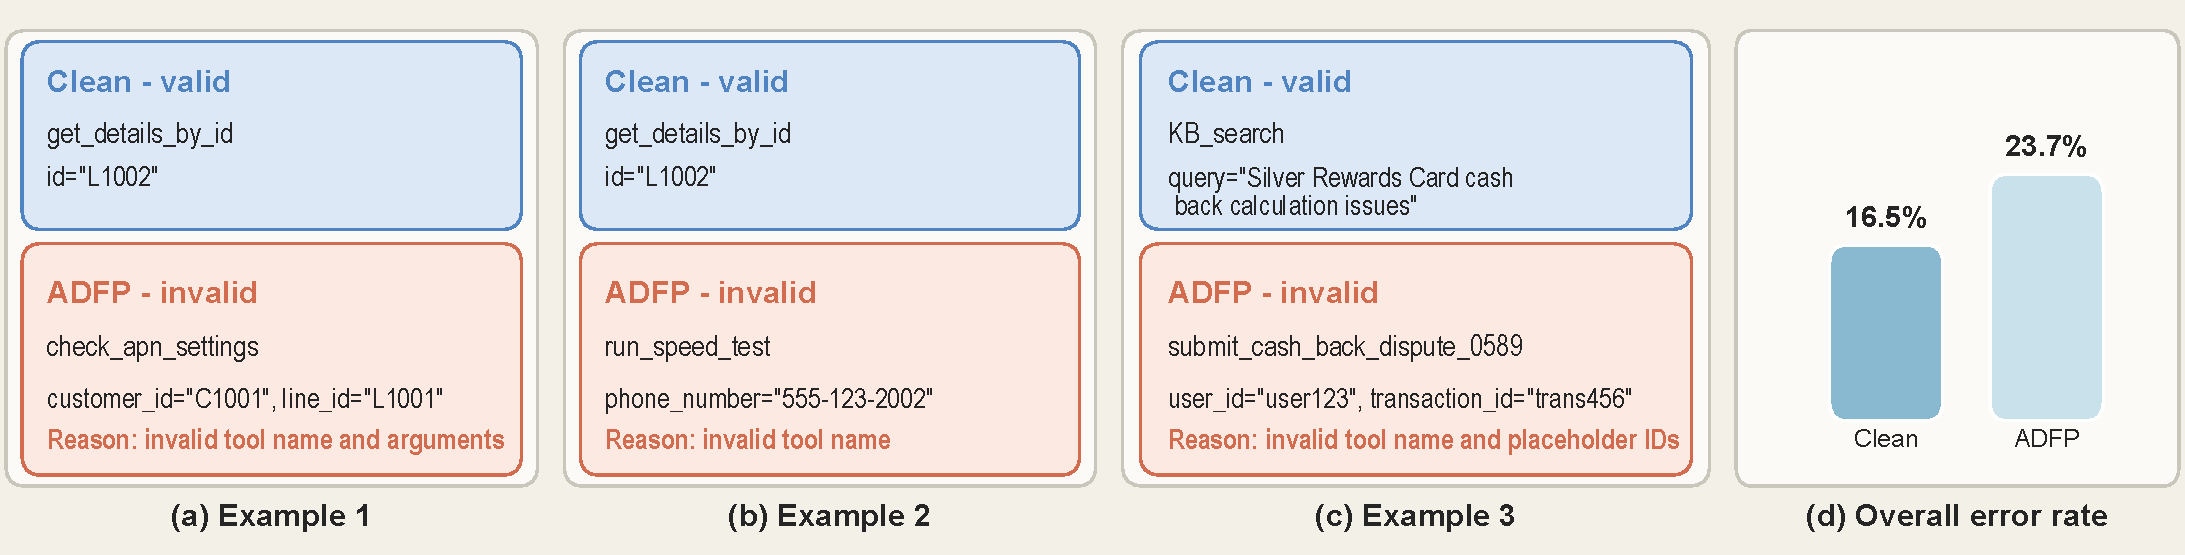
\includegraphics[width=\textwidth]{figure/adfp_agent_utility_failures.pdf}
    \caption{ADFP utility loss. Panels (a)--(c) show three trajectory excerpts,
    each taken from the same-numbered interaction round of the same question.
    The clean trajectory produces a valid tool call, whereas the ADFP trajectory
    invokes a nonexistent tool or uses incorrect arguments. Panel (d) reports
    the overall error rate across all tool calls.}
    \label{fig:adfp-agent-utility}
\end{figure*}

\subsubsection{Limitations of Proactive Watermarking}
Proactive watermarking embeds controlled signals into teacher outputs and can
therefore provide stronger evidence of distillation. However, existing methods
still have limitations in utility, cost, and robustness. ADFP~\cite{xu2026antidistillation} changes the token-sampling process and requires an additional proxy model during decoding. Such token-level changes may corrupt structured outputs in agent settings. We evaluate ADFP with $\lambda=140$ on 20 Tau2 tasks using Qwen3-14B as the teacher and Qwen3-8B as the student. The tool-call error rate increases from $22/133$ ($16.5\%$) in the clean setting
to $31/131$ ($23.7\%$) with ADFP. As shown in Figure~\ref{fig:adfp-agent-utility}, ADFP trajectories may invoke nonexistent tools or produce incorrect arguments. ADFP is also sensitive to data flooding: in the partially fingerprinted data experiment in Section~5.2 and Figure~6 of the original paper, mixing fingerprinted and clean outputs at a 1:1 ratio yields $p>0.05$ in all four unsupervised evaluation settings, so the fingerprint is no longer statistically significant~\cite{xu2026antidistillation}. ADFP is also sensitive to data flooding in Section~5.2 and Figure~6 of the original paper, mixing watermarked data and clean data at a 1:1 ratio yields $p>0.05$ in all four unsupervised evaluation settings, so the fingerprint is no longer statistically significant.

AgentWM~\cite{wang2026protecting} introduces behavioral signals with relatively low embedding cost, but its effectiveness drops greatly when the teacher and
student use different base models. Its signals can also be weakened by
watermark dilution as shown in Table~\ref{tab:baseline-robustness}. AgentGuide~\cite{huang2025agent} and SeqWM~\cite{an2026sequential} require additional watermark embedding or
verification, while their signals may not reliably survive distillation.
As shown by our baseline results in Section~\ref{sec:detection-effectiveness} and Table~\ref{tab:baseline-effectiveness}, AgentWM succeeds only for the GLM-4.7-Flash student, while SeqWM fails to detect any of the tested distilled students. Therefore, existing proactive watermarking methods cannot simultaneously preserve agent utility, remain robust to model and data changes, and keep deployment costs within an acceptable range.


\subsubsection{Limitations of Passive Fingerprinting}
Passive fingerprinting requires no changes to teacher outputs, but its evidence is usually indirect and may not remain stable under model or data changes. PoS Templates~\cite{wadhwa2025taught} relies on syntactic patterns inherited from the teacher, but these patterns may be weakened by further fine-tuning, data augmentation, multi-teacher distillation, or shared training data. Data-Free KD~\cite{shi2026knowledge} requires white-box access to the student model's weights. DistillDetect~\cite{rawat2026reference} relies on student logits and calibrated reference models, making it difficult to use through a standard black-box API. SCOUT~\cite{jang2026retrospective} supports black-box detection, but may confuse related models, and its fingerprints can be overwritten by later training. Therefore, these methods are sensitive to post-training changes and mainly provide indirect similarity-based evidence rather than strong evidence of unauthorized distillation.






\subsection{Vulnerabilities in Token-Level N-gram Matching}
\label{sec:textual-similarity}

\citet{panfilov2026stealing} study visible-answer overlap after prefilling a model's reasoning channel with a short teacher reasoning prefix. Their
Appendix~B.2 evaluates 30 Humanity's Last Exam problems using shared
1-, 2-, and 3-grams against the first 100 tokens of the reference answer,
with best-of-$k$ sampling up to $k=100$. The visible answer is generated
entirely by the target model. Their Figures~11--23 illustrate 13 public
examples with problem statements, teacher reasoning excerpts, and
visible-answer excerpts. Using selected public cases, we test whether
alternative prefixes and shared solution patterns can produce high
overlap with the same teacher reference.

We use a fixed local overlap implementation. For each candidate $a$ and
reference $b$, we tokenize both texts with the same regex tokenizer and
retain up to their first 100 tokens. Let $G_n(x)$ denote the set of distinct
$n$-grams in the retained tokens of $x$. We compute
\begin{equation}
    s_{\mathtt{ngram}}(a,b)
    =
    \frac{\sum_{n=1}^{3}|G_n(a)\cap G_n(b)|}
         {\sum_{n=1}^{3}|G_n(b)|}.
    \label{eq:local-ngram-proxy}
\end{equation}

\partitle{Alternative prefixes and comparisons across model versions}
On the geometry problem in Figure~11 of \citet{panfilov2026stealing},
Kimi-K2.6, which was publicly released before Claude Opus~4.8
\citep{team2025kimi,anthropic2026opus48},
obtains mean/best-of-4 scores of $0.274/0.565$ with the
teacher opening \texttt{This is a known}, compared with $0.373/0.662$
under \texttt{This is an unfamiliar} and $0.250/0.415$ without a prefix.
The best local score of $0.662$ approaches the reported $0.80$ overlap
between prefilled Kimi-K3 and Opus~4.8.
Within this fixed scoring setup, the alternative prefix produces a larger
increase than the authentic prefix across both metrics.
The selected $0.662$ answer shares the opening derivation order $C,F,E,D,B$
with the Opus~4.8 reference, as shown in Figure~\ref{fig:geometry-answer-comparison}.
The sampled Opus~4.6 answers use tables or
different orders; the highest score among these answers is $0.343$ against the
same reference. Thus, this local formatting match is not exclusive to the
teacher prefix or to the sampled Claude-family answers.

\partitle{Convergence on standard solutions}
For the linear differential equation in Figure~13 of
\citet{panfilov2026stealing}, a standard solution uses a $\cosh$ integrating
factor. Without a teacher prefix,
GPT-OSS-120B reaches a mean overlap of $0.500$ and a best-of-4 score of
$0.537$. Kimi-K2.6 similarly scores $0.501$ without a prefix and $0.502$
with the teacher prefix. The unprefilled local scores are numerically close
to the reported $0.50$ overlap between prefilled Kimi-K3 and Opus~4.8.
The unprefilled answer excerpts are shown in Figure~\ref{fig:ode-answer-comparison}.
Our results show that substantial local overlap can arise in standard
solutions with conventional terminology and ordering, while the teacher
prefix adds little in the Kimi-K2.6 comparison.

\partitle{Response steering and sampling}
Visible-answer overlap must also be interpreted in light of how responses
are generated, presented, and selected. In our geometry evaluation of Kimi-K3,
all 20 completions across five prefix
conditions re-derive the solution, and none states the answer within its
first 50 reasoning tokens, unlike the early answer in the reference trace.
Higher visible overlap can therefore coexist with a different observed
reasoning pattern. At the level of answer presentation, even correct
solutions can receive very low scores when little matching text is
available: for the problem in Figure~15 of \citet{panfilov2026stealing},
four correct answers constrained to at most
15 words each score $0.005$. Such sensitivity to presentation also matters
when interpreting best-of-$k$ results, which report the largest overlap
in a sampling pool. Formatting cues can therefore raise the reported score
through occasional high-overlap completions without representing typical
output behavior.
\begin{figure*}[!t]
    \centering
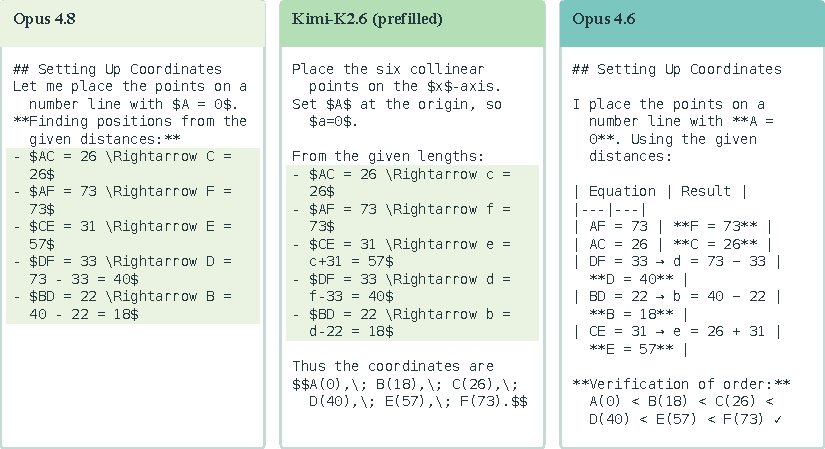
\includegraphics[width=0.72\textwidth]{figure/geometry_answer_comparison.pdf}
    \caption{Excerpts from the original answers to the geometry problem in
    Figure~11 of \citet{panfilov2026stealing}.
    Green shading marks the shared $C,F,E,D,B$ derivation order.
    For each candidate model, we show the highest-overlap answer from four
    samples.}
    \label{fig:geometry-answer-comparison}

    
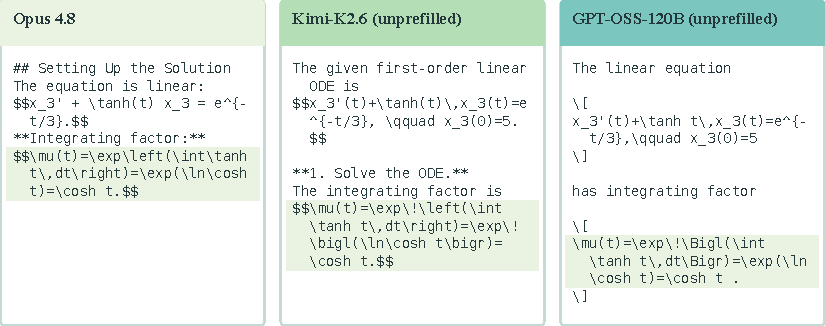
\includegraphics[width=0.72\textwidth]{figure/ode_answer_comparison.pdf}
    \caption{Excerpts from the original answers to the differential-equation
    problem in Figure~13 of \citet{panfilov2026stealing}.
    Green shading marks the shared $\cosh t$ integrating factor.
    Each candidate has the highest reported overlap among four unprefilled
    samples.}
    \label{fig:ode-answer-comparison}
\end{figure*}
\subsection{Vulnerabilities in Agent Execution Graph Similarity}
\label{sec:dependency-ambiguity}
AgentEcho's Action Graph Similarity (AGS) averages optional-tool agreement
$S_{\mathtt{node}}$, sequential-pattern similarity $S_{\mathtt{seq}}$,
and dependency-pattern similarity $S_{\mathtt{dep}}$
\citep{yang2026agents}. Moving from text to tool behavior introduces
structural evidence, but its interpretation depends on which graph
properties the metrics preserve.

\partitle{Scale invariance and structural ambiguity}
For a dependency graph $G$, $S_{\mathtt{dep}}$ compares
$\phi(G)=(r_{\mathtt{reuse}},d_{\mathtt{max}},r_{\mathtt{fanout}})$ by cosine
similarity \citep[Appendix~B.4]{yang2026agents}. These features describe
the fraction of calls after the first that receive dependency inputs,
the longest dependency path, and the fraction of
source nodes with multiple outgoing dependency edges. Cosine similarity
ignores feature-vector magnitude. Consider two graphs with 11 nodes:
one contains a single dependency edge, whereas the other is a complete
10-edge chain. With path length measured in edges,
\begin{equation}
    \phi(G_{\mathtt{single}})=(0.1,1,0),\qquad
    \phi(G_{\mathtt{chain}})=(1,10,0)
    =10\phi(G_{\mathtt{single}}).
    \label{eq:dependency-counterexample}
\end{equation}
Their $S_{\mathtt{dep}}$ is exactly 1 despite large differences in reuse
and dependency depth. Hence, a perfect score does
not guarantee closely matching dependency structures.

\partitle{Evidence from tool trajectories}
We audit 75 trajectories from five models on 15 tasks and compare all
ten model pairs within each task, yielding 150 comparisons.
The mean $S_{\mathtt{dep}}$ is $0.885$,
and 121 comparisons score at least $0.9$. Among these, 53 have dependency
edge counts differing by at least three, and 49 pair a successful
trajectory with a failed one. In \texttt{retail-37}, a failed trajectory
with one dependency edge and a successful trajectory with 12 edges score
$0.991$. We further verify candidate dependency edges with an LLM judge,
using anonymized values and a prompt adapted from the published protocol
\citep[Appendix~B.1]{yang2026agents}.
Both the score and the edge-count discrepancy remain unchanged for this
example.
Thus, near-perfect dependency similarity persists despite substantial
structural differences, even after LLM-based edge verification.

\partitle{Behavioral convergence after reasoning distillation}
\label{sec:reasoning-distillation-convergence}
Inspired by the reference-based formulation of \citet{rawat2026reference},
we measure changes in behavioral similarity relative to the base checkpoint.
We use the Qwen3.5-9B base model as the reference checkpoint and evaluate
its publicly released reasoning-distilled variant.\footnote{Model card:
\href{https://huggingface.co/Jackrong/Qwen3.5-9B-Claude-4.6-Opus-Reasoning-Distilled-v2-GGUF}{Jackrong's
reasoning-distilled Qwen3.5-9B (GGUF)}.}
The model card identifies Claude Opus~4.6 as the teacher.
Our audit of 12,592 publicly available examples from the model card's
listed datasets finds no structured tool trajectories.
We use the same agent harness
and user simulator for 15 $\tau$-bench-style tasks, with one rollout per
model and task. Claude Sonnet~4.5 (thinking), Kimi-K2 (thinking), and
GPT-OSS-120B serve as comparison models.

\begin{table}[!t]
    \centering
    \scriptsize
    \setlength{\tabcolsep}{2pt}
    \resizebox{\columnwidth}{!}{%
    \begin{tabular}{lrrrrrr}
        \hline
        Comparison model & AGS$_{\mathtt{base}}$ & AGS$_{\mathtt{dist}}$
        & $\Delta\mathtt{AGS}$ & $\Delta S_{\mathtt{node}}$
        & $\Delta S_{\mathtt{seq}}$ & $\Delta S_{\mathtt{dep}}$ \\
        \hline
        Claude Sonnet~4.5 (thinking) & 0.549 & 0.709 & +0.160 & $-0.031$ & +0.425 & +0.086 \\
        Kimi-K2 (thinking) & 0.561 & 0.850 & +0.289 & +0.042 & +0.750 & +0.077 \\
        GPT-OSS-120B & 0.584 & 0.770 & +0.186 & $-0.047$ & +0.525 & +0.080 \\
        \hline
    \end{tabular}
    }
    \caption{Changes in AGS and its components after reasoning
    distillation on the same 15 tasks.
    Component values are rounded independently.}
    \label{tab:reasoning-distillation-similarity}
\end{table}

Table~\ref{tab:reasoning-distillation-similarity} shows that AGS increases
toward all three models, alongside a rise in task success from
$4/15$ to $12/15$. The gains are dominated by $S_{\mathtt{seq}}$, which
increases by $0.425$--$0.750$.
In contrast, $S_{\mathtt{dep}}$ increases by $0.077$--$0.086$, while
$S_{\mathtt{node}}$ decreases toward both Claude and GPT-OSS.
Thus, these gains primarily reflect convergence in local execution
statistics and do not uniquely identify teacher-specific tool-use inheritance.

\partitle{Implications for attribution}
These cases expose ambiguity in interpreting high unwatermarked similarity
as evidence of a specific training source. They motivate controls for shared
solutions, response presentation, and general behavioral improvement,
alongside calibrated false-positive rates. Our watermarking framework
provides private verification signals tied to recorded teacher interactions.

\section{Detailed Watermarking Protocols}

\begin{figure*}[!t]
\hrule width \hsize \kern 1mm \hrule width \hsize height 2pt 

\textbf{\name{} Watermark Embedding Protocol}

\hrule

\small
\textbf{Inputs:} Tool schema $\mathcal{F}$, Secret key $k$, Trajectory ID $\mathtt{id}_\tau$, Hyperparameters $(p_0, \Delta p, p_{\mathtt{max}}, B, K)$. \\
\textbf{Outputs:} Watermarked trajectory $\tau$, Private evidence card set $\mathcal{C}_\tau$.


\noindent \textbf{1. Initialization Phase:} 
\begin{itemize}
    \item \textit{System Setup:} 
    \begin{itemize}
        \item Evaluate the tool schema $\mathcal{F}$ using the safety model $\mathcal{M}_{\mathtt{safe}}$ to obtain the valid subset $\mathcal{F}_{\mathtt{safe}}$.
        \item Initialize the dynamic trigger probability $p_1 = p_0$, the remaining budget $b_1 = B$, and an empty evidence set $\mathcal{C}_\tau = \emptyset$.
    \end{itemize}
\end{itemize}

\noindent \textbf{2. Real-Time Embedding Phase:} \\
For each step $t$ immediately following a completed core action $a_{\mathtt{core}}^{t-1}$, the system executes:
\begin{itemize}
    \item \textit{Dynamic Scheduling:}
    \begin{itemize}
        \item Compute a cryptographic hash $u_t = \mathtt{Hash}(k \parallel a \parallel \mathtt{id}_\tau \parallel t) \in [0, 1)$.
        \item If the budget is none ($b_t = 0$) or the condition is not met ($u_t \ge p_t$), skip and failure update.
    \end{itemize}
    
    \item \textit{Candidate Generation \& Scoring:}
    \begin{itemize}
        \item Generate $K$ auxiliary candidates $(t_{\mathtt{aux}}^j, a_{\mathtt{aux}}^j)_{j=1}^K$ using the teacher model $\mathcal{M}_t$ and filter them through the validation mechanism.
        \item For each valid candidate $(t_{\mathtt{aux}}^j, a_{\mathtt{aux}}^j)$, compute the score $S_j$ based on naturalness ($s_{\mathtt{rel}}^j$), logical consistency ($s_{\mathtt{relb}}^j$), and repeatability $s_{\mathtt{relb}}^j$ for the tool pairing $(f_{\mathtt{core}}, f_{\mathtt{aux}}^j)$.
        \item Select the candidate with the highest score as $(t_{\mathtt{aux}}^{\mathtt{best}}, a_{\mathtt{aux}}^{\mathtt{best}})$. If no valid candidates exist, skip to the failure update.
    \end{itemize}

    \item \textit{Injection \& Success Update:}
    \begin{itemize}
        \item Inject $(t_{\mathtt{aux}}^{\mathtt{best}}, a_{\mathtt{aux}}^{\mathtt{best}})$ into the trajectory to receive the auxiliary observation $o_{\mathtt{aux}}^{\mathtt{best}}$.
        \item Reset the probability $p_{t+1} = p_0$ and decrement the budget $b_{t+1} = b_t - 1$.
        \item Increment the historical repeat count for this specific tool pairing $(f_{\mathtt{core}}, f_{\mathtt{aux}}^{\mathtt{best}})$.
        \item Create an evidence card $c_t = (h, t_{\mathtt{core}}^{t-1}, a_{\mathtt{core}}^{t-1}, o_{\mathtt{core}}^{t-1}, f_{\mathtt{aux}}^{\mathtt{best}}, p_{\mathtt{aux}}^{\mathtt{best}})$ and append it to $\mathcal{C}_\tau$.
    \end{itemize}

    \item \textit{Failure/Skip Update (Executed only if no injection occurred):}
    \begin{itemize}
        \item Increase the trigger probability $p_{t+1} = \min\{p_t + \Delta p, p_{\mathtt{max}}\}$ to boost future injection chances, and retain the current budget $b_{t+1} = b_t$.
    \end{itemize}
\end{itemize}

\hrule width \hsize \kern 1mm \hrule width \hsize height 2pt 
\caption{The watermark embedding protocol of \name{}. }
\label{fig:watermark_embedding_protocol}
\end{figure*}

\begin{figure*}[!t]
\hrule width \hsize \kern 1mm \hrule width \hsize height 2pt 

\textbf{\name{} Watermark Detection Protocol}

\hrule

\small
\textbf{Inputs:} Combined evidence pool $\mathcal{C}_{\mathcal{S}}$, Suspect model $\mathcal{M}_s$, Teacher model $\mathcal{M}_t$, Hyperparameters $(p, r, N)$. \\
\textbf{Outputs:} Detection decision $\in \{\mathtt{True}, \mathtt{False}\}$, and the statistical $p\mathtt{-value}$.


\noindent \textbf{1. Probe Construction Phase:} \\
For each evidence card $c_i \in \mathcal{C}_{\mathcal{S}}$, the system executes:
\begin{itemize}
    \item \textit{Paired Probes Generation:}
    \begin{itemize}
        \item Generate up to $N_i$ parameterized variants using card $c_i$ to form the real probe set $p_{\mathtt{real}}^i$.
        \item Construct the corresponding fake probe set $p_{\mathtt{fake}}^i$ by replacing the core action in $p_{\mathtt{real}}^i$ with a semantically altered fake core.
    \end{itemize}
\end{itemize}

\noindent \textbf{2. Evaluation Phase:} \\
For each probe variant $j \in [1, N_i]$ of card $c_i$, the system executes:
\begin{itemize}
    \item \textit{Target Model Query \& Parsing:}
    \begin{itemize}
        \item Submit the real probe $p_{\mathtt{real}, j}^i$ to the suspect model $\mathcal{M}_s$ and parse the output to compute the strict fullhit indicator $h_{i,j}^{\mathtt{real}} \in \{0, 1\}$.
        \item Submit the fake probe $p_{\mathtt{fake}, j}^i$ to the suspect model $\mathcal{M}_s$ and parse the output to compute the strict fullhit indicator $h_{i,j}^{\mathtt{fake}} \in \{0, 1\}$.
    \end{itemize}
\end{itemize}

\noindent \textbf{3. Card-Level Aggregation Phase:} \\
For each card $c_i \in \mathcal{C}_{\mathcal{S}}$, the system executes:
\begin{itemize}
    \item \textit{Hit Rate \& Performance Calculation:}
    \begin{itemize}
        \item Compute the hit rates across all $N_i$ variants: $R_i^{\mathtt{real}} = \frac{1}{N_i} \sum_{j} h_{i,j}^{\mathtt{real}}$ and $R_i^{\mathtt{fake}} = \frac{1}{N_i} \sum_{j} h_{i,j}^{\mathtt{fake}}$.
        \item Calculate the performance difference: $\Delta_i = R_i^{\mathtt{real}} - R_i^{\mathtt{fake}}$.
        \item Tally the results: increment the real win count $w$ if $\Delta_i > 0$, and increment the fake win count $\ell$ if $\Delta_i < 0$ (ties where $\Delta_i = 0$ are excluded).
    \end{itemize}
\end{itemize}

\noindent \textbf{4. Statistical Test \& Decision Phase:} 
\begin{itemize}
    \item \textit{Hypothesis Testing:}
    \begin{itemize}
        \item Compute the one-sided exact sign-test $p\mathtt{-value} = \sum_{k=w}^{w+\ell}\binom{w+\ell}{k}2^{-(w+\ell)}$.
        \item Compute the global mean difference $\Delta_{\mathtt{mean}} = \frac{1}{|\mathcal{C}_{\mathcal{S}}|} \sum_{i} \Delta_i$.
    \end{itemize}
    
    \item \textit{Dual Criteria Check:}
    \begin{itemize}
        \item Output $\mathtt{True}$ (Detection Successful) if both $p\mathtt{-value} < p$ and $\Delta_{\mathtt{mean}} \ge r$ hold. Otherwise, output $\mathtt{False}$.
    \end{itemize}
\end{itemize}

\hrule width \hsize \kern 1mm \hrule width \hsize height 2pt 
\caption{The watermark detection protocol of \name{}.}
\label{fig:watermark_detection_protocol}
\end{figure*}




